\section{Box-counting dimenze}\label{sec:box-counting-dimenze}

Tomuto typu dimenze jsme se již v základu věnovali v kapitole \ref{chapter:uvod_do_fraktalu}, specificky sekci \ref{sec:fraktalni_dimenze}, kde jsme rozebrali jeho způsob jejího výpočtu a ukázali jsme si jej několika příkladech. V této části si blíže rozebereme některé další vlastnosti týkající se právě \emph{box-counting dimenze}\index{box-counting dimenze}\footnote{V kapitole \ref{chapter:uvod_do_fraktalu} jsme pro jednoduchost používali obecnější termín \emph{fraktální dimenze}. Ten však zahrnuje daleko širší škálu možných definic, než jen tu, kterou jsme si představili. Avšak dále v tomto textu budeme používat výhradně její skutečný název, tj. box-counting dimenze.} a pokusíme se ji lépe zasadit do kontextu teorie míry, které jsme se samostatně až do této chvíle věnovali.

Jako první se podíváme na myšlenku box-counting trochu blíže a maličko si ji zobecníme. Původně jsme nahlíželi na dimenzi jako na exponent, s nímž roste "velikost" zkoumaného útvaru. Tato myšlenka nás se ukázala jako rozumná, neboť pro "klasické" geometrické útvary vycházela tato dimenze vždy celočíselně, nicméně už tomu tak nebylo v případě fraktálních útvarů. Myšlenka byla taková, že jsme útvar $F$ rozdělili na určitý počet stejně "velkých částí", označme $F_1,F_2,\ldots,F_m$, v nějakém měřítku $\varepsilon>0$. Zkusme nyní požadavek na striktně stejnou velikost (formálně vzato míru) trochu rozvolnit. Bude nám stačit, když pro každé $i$ je $\diam{F_i}\leqslant\delta$, kde $\delta>0$. Zároveň nebudeme požadovat, aby množiny $F_1,F_2,\ldots,F_m$ byly všechny striktně po dvou téměř disjunktními\footnote{Množiny $M,N$ jsou \emph{téměř disjunktní}, pokud $\interior{M}\cap\interior{N}=\emptyset$, tedy může nastat, že se na hranici mohou "dotýkat", tzn. $\boundary{M}\cap\boundary{N}\neq\emptyset$.} podmnožinami $F$, ale stačí, když budou tvořit pokrytí $F$.

Mějme tedy nějakou neprázdnoou omezenou množinu $F\subset\R^n$, kde pro každé $\delta>0$ budeme hledat \emph{nejmenší počet} množin, takových, že pokrývají $F$. Toto číslo si označíme $N_\delta(F)$. Dimenze množiny $F$ by tedy měla odrážet "rychlost" růstu $N_\delta(F)$ pro $\delta\to 0^+$. Je-li splněna aproximace
\begin{equation}\label{eq:odhad-n-delta}
    N_\delta(F)\approx c\delta^{-s}
\end{equation}
pro $c>0$, pak řekneme, že množina $F$ má box-counting dimenzi $s$. (Převzato z \citep[str. 27]{Falconer2014}.)
\begin{remark}
    V dalším textu budeme místo $\delta\to 0^+$ psát pro jednoduchost pouze $\delta\to 0$, byť by se slušilo používat první variantu. Čtenáři je však nejspíše jasné, že uvažovat záporný průměr množiny nemá smysl.
\end{remark}
Logaritmováním a úpravou výrazu \eqref{eq:odhad-n-delta} dostaneme:
\begin{align}\label{eq:odvozeni-box-counting-dimenze}
    \ln{N_\delta(F)}&\approx\ln{c}+\ln{\delta^{-s}}\\
    \ln{N_\delta(F)}&\approx\ln{c}-s\ln{\delta}\\
    s&\approx\dfrac{\ln{N_\delta(F)}}{-\ln{\delta}}+\dfrac{\ln{c}}{\ln{\delta}}.
\end{align}
Když porovnáme výsledek v \eqref{eq:odvozeni-box-counting-dimenze} s rovností \eqref{eq:fraktalni-dimenze} z minulé kapitoly, můžeme si všimnout, že zde navíc figuruje člen $\ln{c}/\ln{\delta}$. Když však uvážíme limitu daného výrazu pro $\delta\to 0$, dostaneme původní vzorec, který jsme již viděli, tj.
\[\lim_{\delta\to 0}\left(\dfrac{\ln{N_\delta(F)}}{-\ln{\delta}}+\dfrac{\ln{c}}{\ln{\delta}}\right)=\lim_{\delta\to 0}\dfrac{\ln{N_\delta(F)}}{-\ln{\delta}}+\lim_{\delta\to 0}\dfrac{\ln{c}}{\ln{\delta}}=\lim_{\delta\to 0}\dfrac{\ln{N_\delta(F)}}{-\ln{\delta}}.\]
% \begin{definition}[$\delta$-pokrytí]\label{def:delta-pokryti}
%     Nechť $(X,\rho)$ je metrický prostor, $F\subseteq X$ a $\delta>0$. Jestliže $\mathcal{F}=\set{F_1,F_2,\ldots}\subseteq\powset{X}$ je pokrytí $F$ a zároveň $\diam{F_j}\leqslant\delta$ pro každé $j$, pak $\mathcal{F}$ nazýváme $\delta$-pokrytí\index{$\delta$-pokrytí} množiny $F$.
% \end{definition}
Předchozí úvahu můžeme shrnout do následující definice.
\begin{definition}[Box-counting dimenze]\label{def:box-counting-dimenze}
    Nechť $F\subset \R^n$ je neprázdná omezená množina. Pak definujeme následující:
    \begin{itemize}
        \item \emph{Nejmenší počet množin v $\delta$-pokrytí množiny $F$} značíme $N_\delta(F)$, tj.
        \[N_\delta(F)=\inf\set{m\;\middle|\;F\subseteq\bigcup_{i=1}^n F_i\;,\;\diam{F_j}\leqslant\delta\;\text{pro}\;1\leqslant j\leqslant m}.\]
        \item \emph{Horní box-counting dimenze} množiny $F$ je
        \[\upperdimB{F}=\limsup_{\delta\to 0}\dfrac{\ln{N_\delta(F)}}{-\ln{\delta}}.\]
        \item \emph{Dolní box-counting dimenze} množiny $F$ je
        \[\lowerdimB{F}=\liminf_{\delta\to 0}\dfrac{\ln{N_\delta(F)}}{-\ln{\delta}}.\]
    \end{itemize}
    V případě, že $\lowerdimB{F}=\upperdimB{F}$, pak společnou hodnotu nazýváme \emph{box-counting dimenzí} množiny $F$, značíme $\dimB{F}$, přičemž platí
    \[\dimB{F}=\lim_{\delta\to 0}\dfrac{\ln{N_\delta(F)}}{-\ln{\delta}}.\]
\end{definition}
\begin{remark}
    Zde je důležité zmínit, že pro v dalším textu budeme uvažovat $\delta$ dostatečně malé, takové, že hodnota $-\ln{\delta}$ je vždy kladná. Dále též budeme pracovat (podle definice \ref{def:box-counting-dimenze}) pouze s neprázdnými omezenými množinami, abychom se vyhnuli problémům s případy, kdy $N_\delta(F)=\infty$ nebo $N_\delta(F)=0$.
\end{remark}
Abychom uvedli vše na pravou míru, box-counting dimenzi lze taktéž definovat více způsoby. V tuto uvažujeme obecně $\delta$-pokrytí dané množiny $F$, tj. pokrytí \emph{obecnými} množinami o průměru maximálně $\delta>0$. Lze se však zaměřit i na konkrétní útvary, jak ukazuje následující věta.
\begin{theorem}[Ekvivalentní definice box-counting dimenze]\label{thm:ekvivalentni-def-box-counting-dimenze}
    Nechť $F\subset \R^n$ je neprázdná omezená množina. Pak
    \begin{align*}
        \lowerdimB{F}&=\liminf_{\delta\to 0}\dfrac{\ln{M_\delta(F)}}{-\ln{\delta}},\\
        \upperdimB{F}&=\limsup_{\delta\to 0}\dfrac{\ln{M_\delta(F)}}{-\ln{\delta}},\\
        \dimB{F}&=\lim_{\delta\to 0}\dfrac{\ln{M_\delta(F)}}{-\ln{\delta}},
    \end{align*}
    kde pro $M_\delta(F)$ platí
    \begin{enumerate}[label=(\roman*)]
        \item\label{thm:pokryti-delta-uz-koulemi} $\displaystyle M_\delta(F)=\inf\set{m\;\middle|\;F\subseteq\bigcup\limits_{i=1}^m K_\delta(x_i)\;,\;x_j\in\R^n\;\text{pro}\;1\leqslant j\leqslant m}$,
        \item\label{thm:pokryti-delta-kvadry} $\displaystyle M_\delta(F)=\inf\set{m\;\middle|\;F\subseteq\bigcup\limits_{i=1}^m I_i\;,\;I_j=\prod_{k=1}^{n}\langle a_k,a_k+\delta\rangle\;\text{pro}\;1\leqslant j\leqslant m}$,
        \item\label{thm:pokryti-delta-sit} $\displaystyle M_\delta(F)=\left|\set{I\;\middle|\;I\cap F\neq\emptyset\;,\;I\in\mathcal{D}}\right|$, kde $\mathcal{D}$ je $\delta$-síť.
        \item\label{thm:pokryti-delta-dis-ot-koulemi} $\displaystyle M_\delta(F)=\sup\set{m\;\middle|\;B_\delta(x_i)\cap B_\delta(x_j)=\emptyset\;;\;x_i,x_j\in\R^n\;\text{pro}\;1\leqslant i,j\leqslant m}$.
    \end{enumerate}
\end{theorem}
(Převzato z \citep[str. 30]{Falconer2014}.)

Pojďme si větu \ref{thm:ekvivalentni-def-box-counting-dimenze} nyní trochu rozebrat.
\begin{itemize}
    \item Body \ref{thm:pokryti-delta-uz-koulemi} a \ref{thm:pokryti-delta-dis-ot-koulemi} říkájí, že $N_\delta(F)$ je rovno \emph{nejmenšímu počtu uzavřených koulí o poloměru $\delta$, které pokrývají $F$}, resp. \emph{nejvyšší počet disjunktních otevřených koulí, které mají střed v $F$}.
    \item Podobně body \ref{thm:pokryti-delta-kvadry} a \ref{thm:pokryti-delta-sit} tvrdí, že $N_\delta(F)$ lze ekvivalentně definovat jako pokrytí kvádry o stranách délky $\delta$, resp. počet všech kvádrů z $\delta$-sítě, které mají s $F$ neprázdný průnik.
\end{itemize}
Pro představu viz obrázek \ref{fig:ilustrace-definic-bc-dimenze}.
\begin{figure}[h]
    \centering
    \begin{subfigure}{0.4\textwidth}
        \centering
        
\includegraphics{ch02-bc-dimenze.pdf}
        \caption{Množina $B=\bigcup_{i=1}^4 B_i$}
        \label{subfig:bc-dimenze-pokryvana-mnozina}
    \end{subfigure}
    \qquad
    \begin{subfigure}{0.4\textwidth}
        \centering
        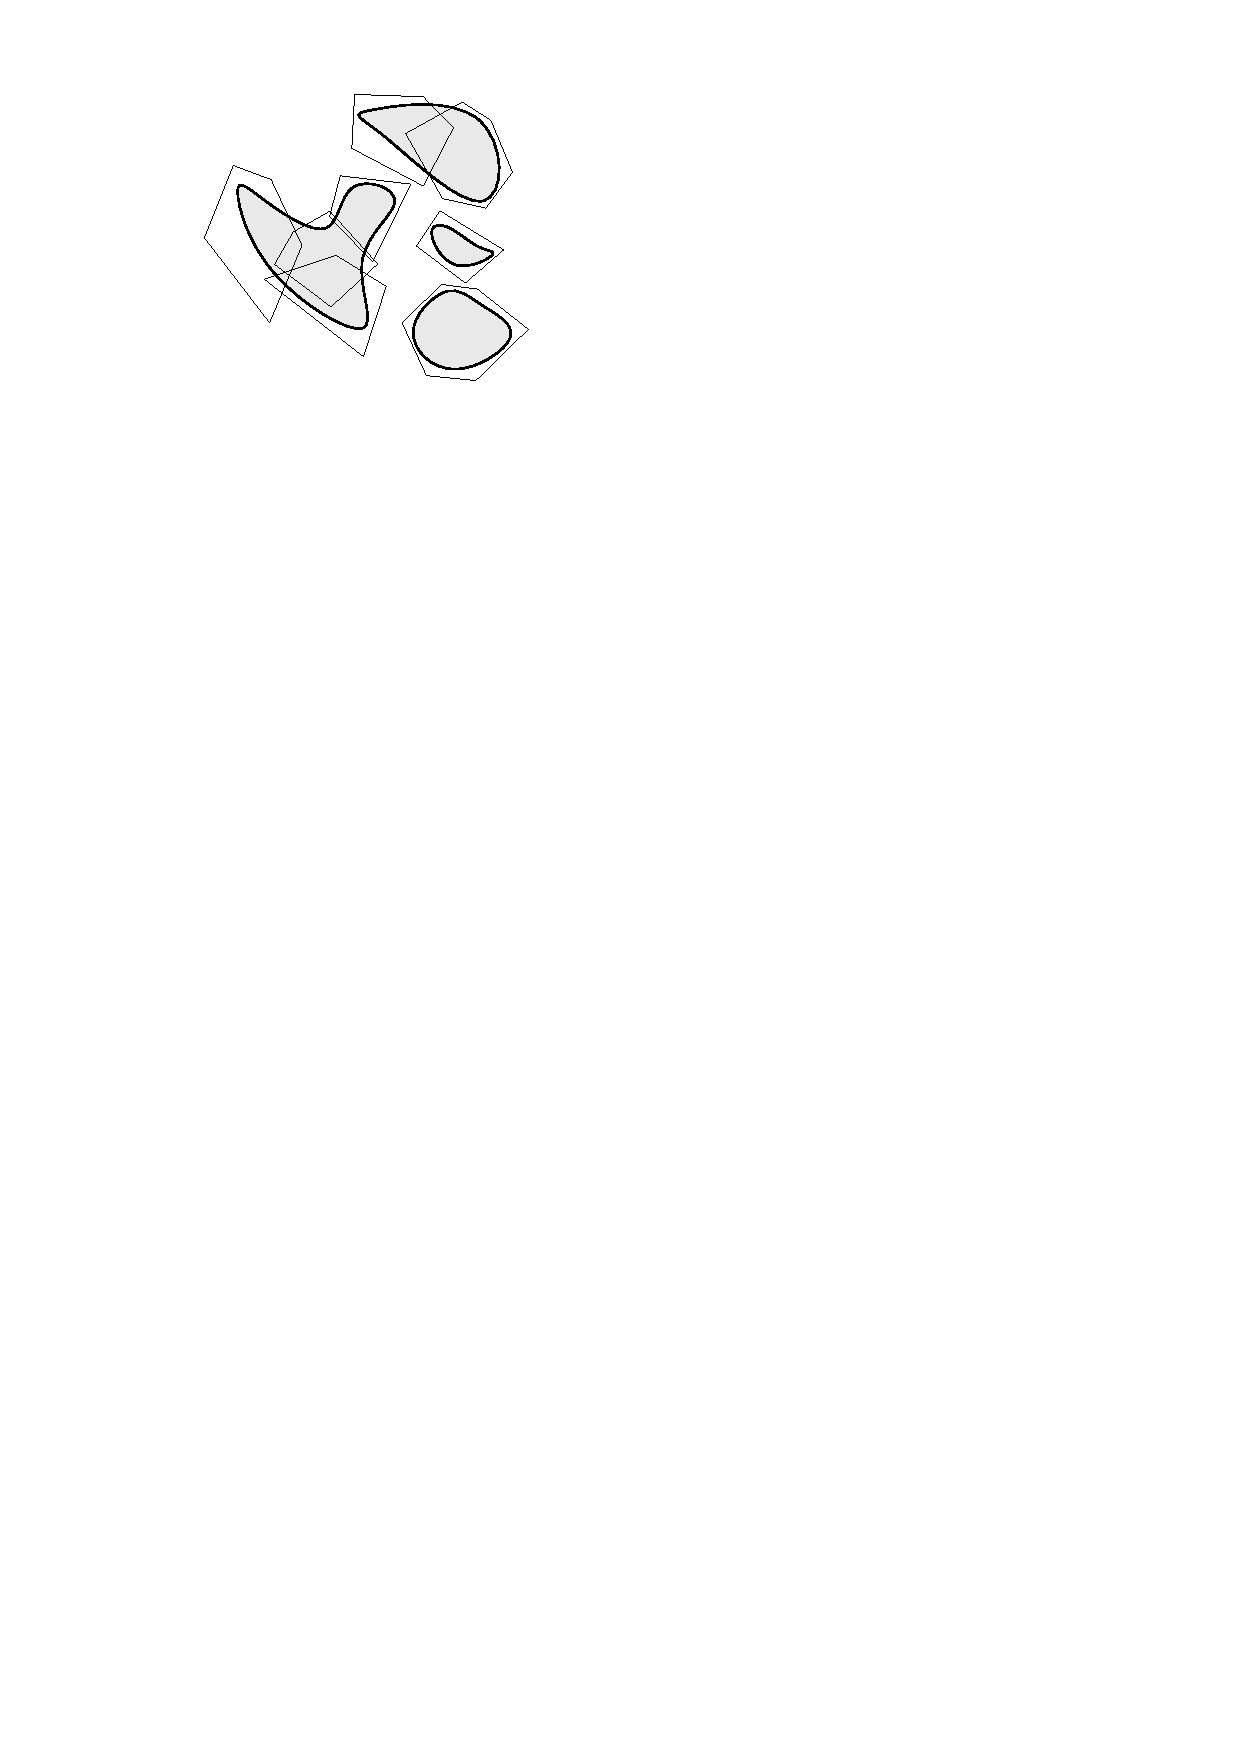
\includegraphics{ch02-bc-dimenze-delta-pokryti.pdf}
        \caption{$\delta$-pokrytí množiny $B$ (viz definice \ref{def:box-counting-dimenze})}
        \label{subfig:bc-dimenze-delta-pokryti}
    \end{subfigure}
    \qquad
    \begin{subfigure}{0.4\textwidth}
        \centering
        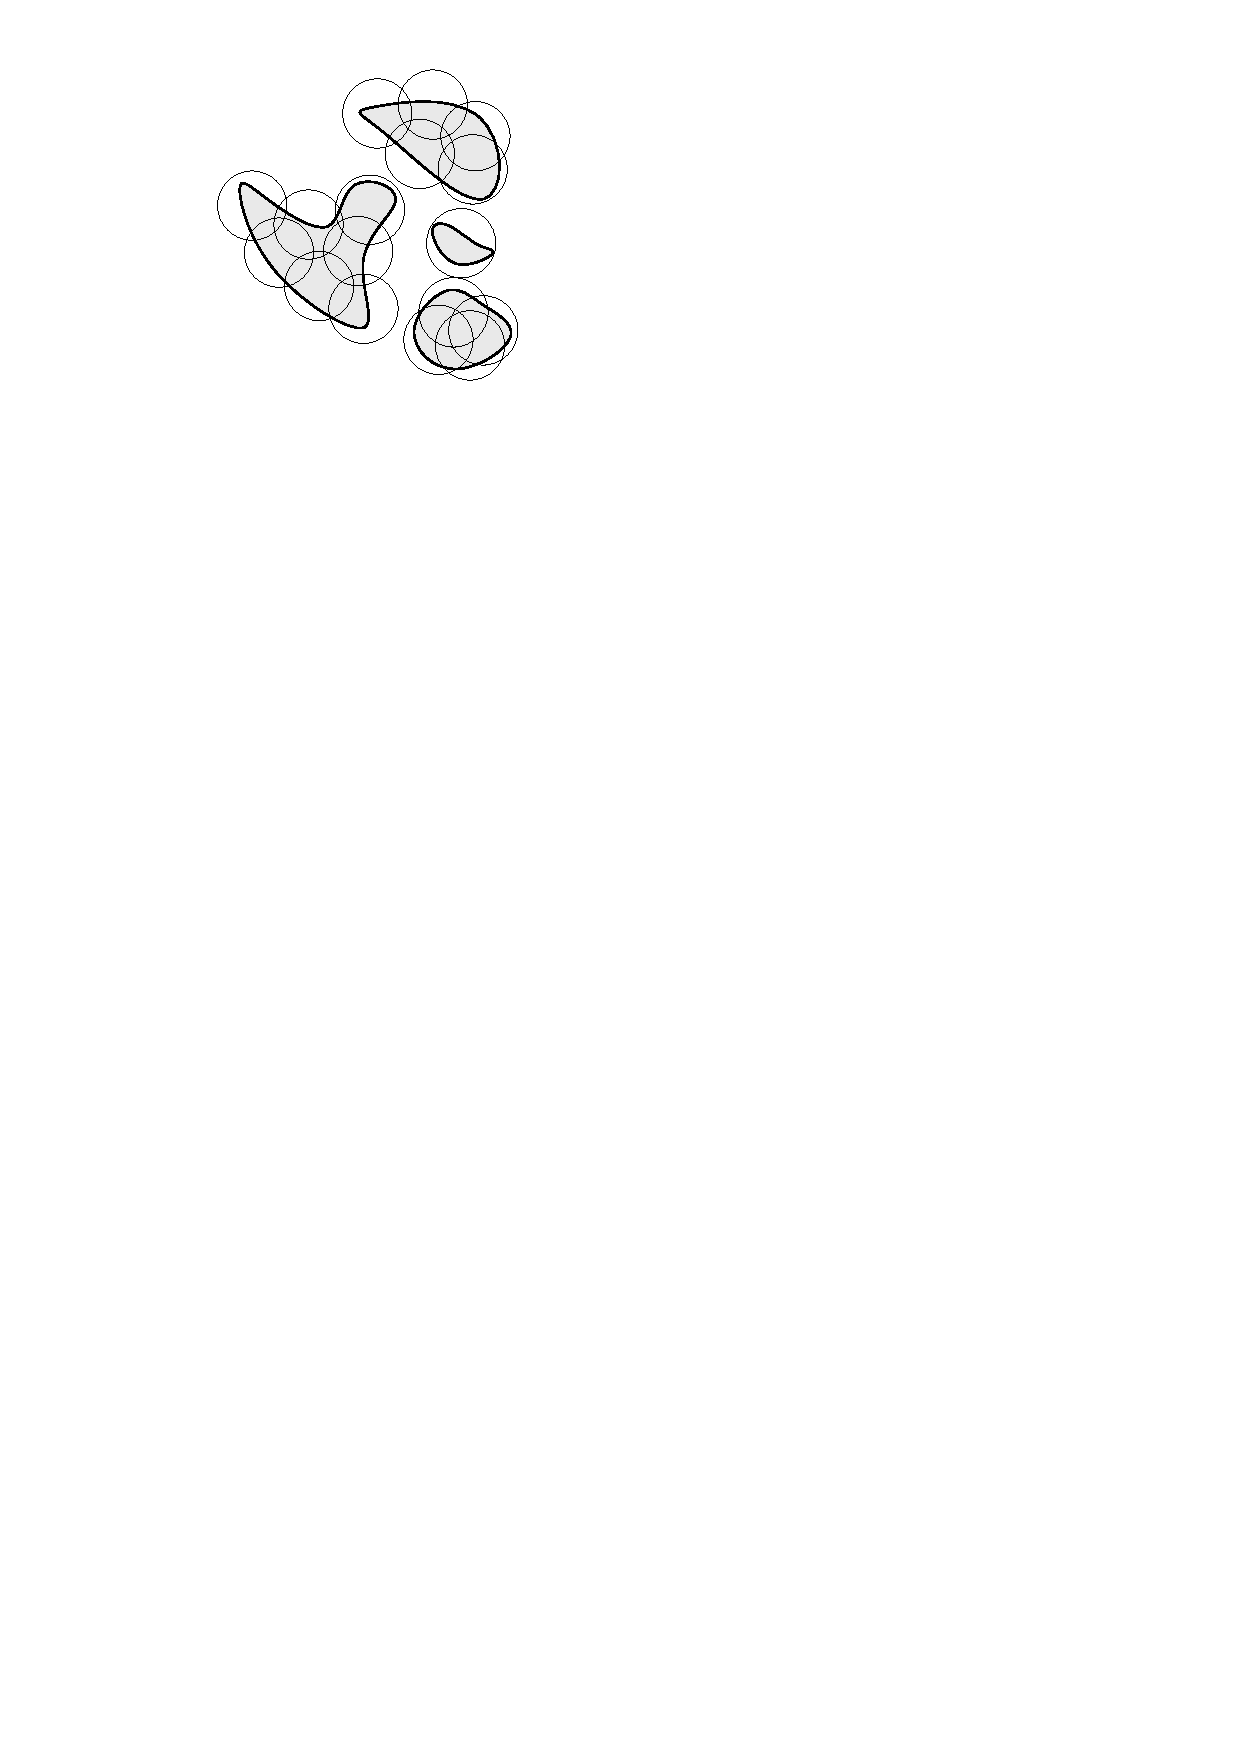
\includegraphics{ch02-bc-dimenze-pokryti-uz-koule.pdf}
        \caption{Pokrytí uzavřenými koulemi (viz bod \ref{thm:pokryti-delta-uz-koulemi})}
        \label{subfig:bc-dimenze-uz-koule}
    \end{subfigure}
    \qquad
    \begin{subfigure}{0.4\textwidth}
        \centering
        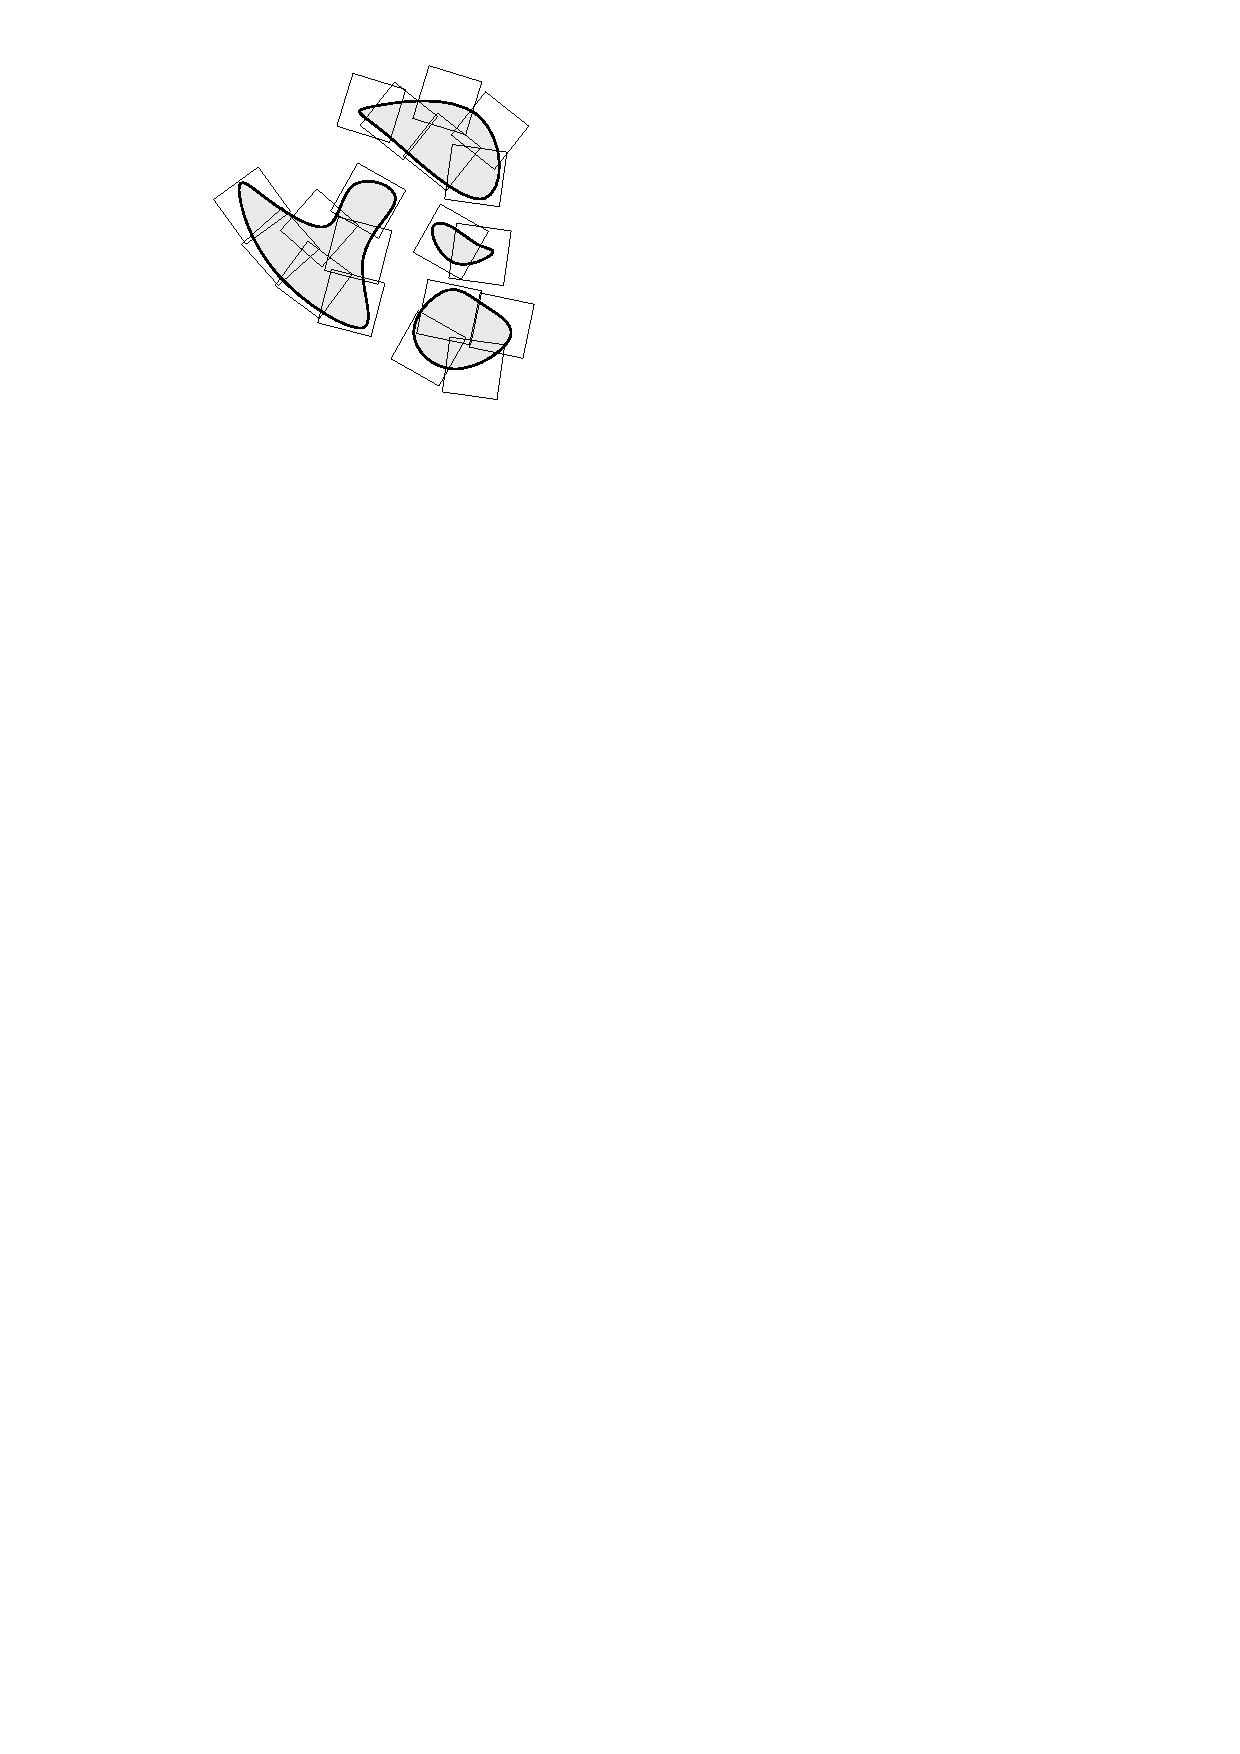
\includegraphics{ch02-bc-dimenze-pokryti-kvadry.pdf}
        \caption{Pokrytí pomocí kvádrů (viz bod \ref{thm:pokryti-delta-kvadry})}
        \label{subfig:bc-dimenze-kvadry}
    \end{subfigure}
    \qquad
    \begin{subfigure}{0.4\textwidth}
        \centering
        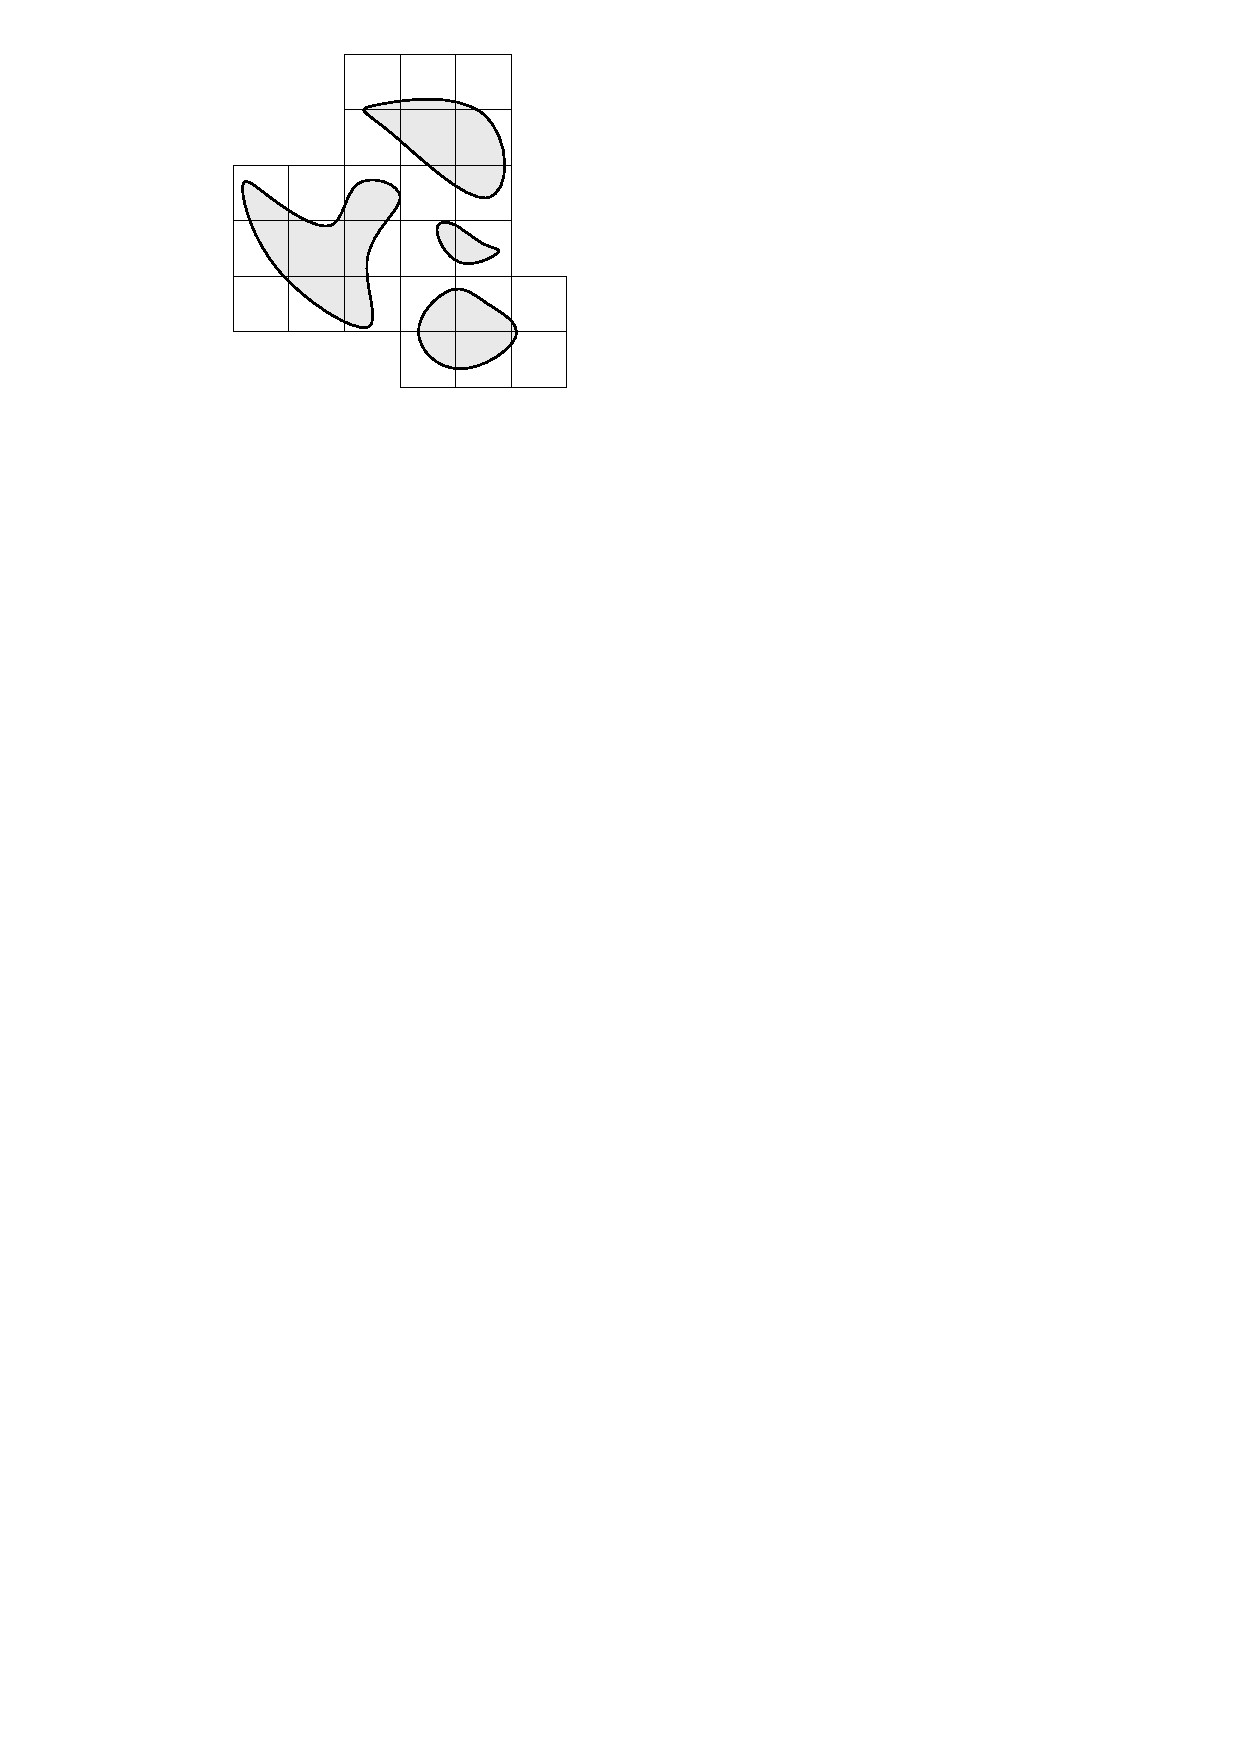
\includegraphics{ch02-bc-dimenze-pokryti-delta-sit.pdf}
        \caption{$\delta$-síť (viz bod \ref{thm:pokryti-delta-sit})}
        \label{subfig:bc-dimenze-delta-sit}
    \end{subfigure}
    \qquad
    \begin{subfigure}{0.4\textwidth}
        \centering
        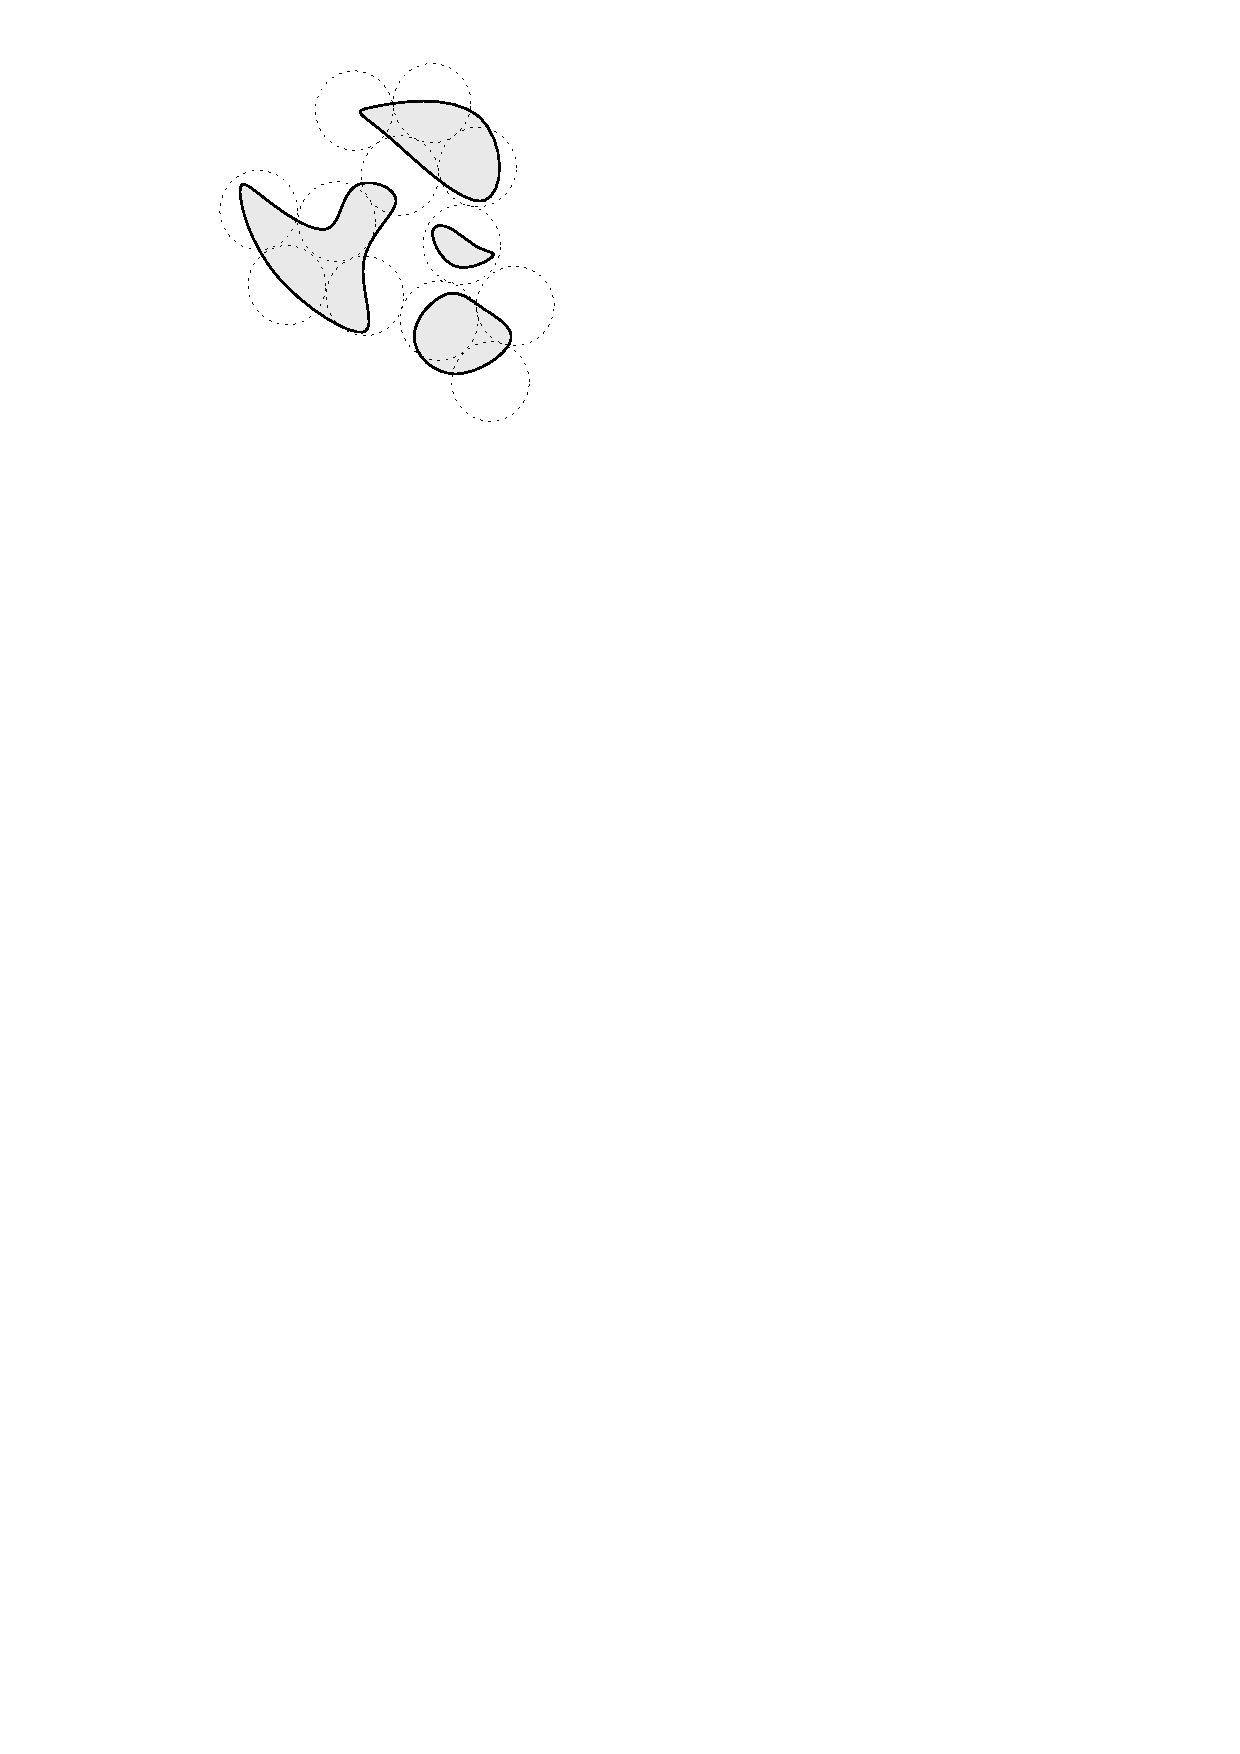
\includegraphics{ch02-bc-dimenze-pokryti-ot-koule.pdf}
        \caption{Pokrytí otevřenými po dvou disjunktními koulemi (viz bod \ref{thm:pokryti-delta-dis-ot-koulemi})}
        \label{subfig:bc-dimenze-ot-koule}
    \end{subfigure}
    \caption{Ilustrace věty \ref{thm:ekvivalentni-def-box-counting-dimenze} (Inspirováno \citep[str. 29]{Falconer2014})}
    \label{fig:ilustrace-definic-bc-dimenze}
\end{figure}

Zároveň body \ref{thm:pokryti-delta-kvadry} a \ref{thm:pokryti-delta-sit} nám dávají dobré opodstatnění názvu tohoto typu dimenze, neboť v podstatě zkoumáme pokrývání daného obrazce "kostkami". Při aproximacích box-counting dimenze obrazce $F\subset\R^2$ tak lze pracovat s mřížkou čtverců o libovolné straně $\delta>0$, kdy $N_\delta(F)$ stanovíme jako počet čtverců, které se překrývají se zkoumaným obrazcem $F$. Když se tedy zpět vrátíme k otázce rozebírané v úvodu tohoto textu týkající se délky pobřeží (viz kapitola \ref{chapter:uvod_do_fraktalu}), lze jeho "fráktálnost" do jisté míry vyjádřit právě popsaným způsobem (viz obrázek \ref{fig:aproximace-delky-pobrezi-vb}).
\begin{figure}[h]
    \centering
    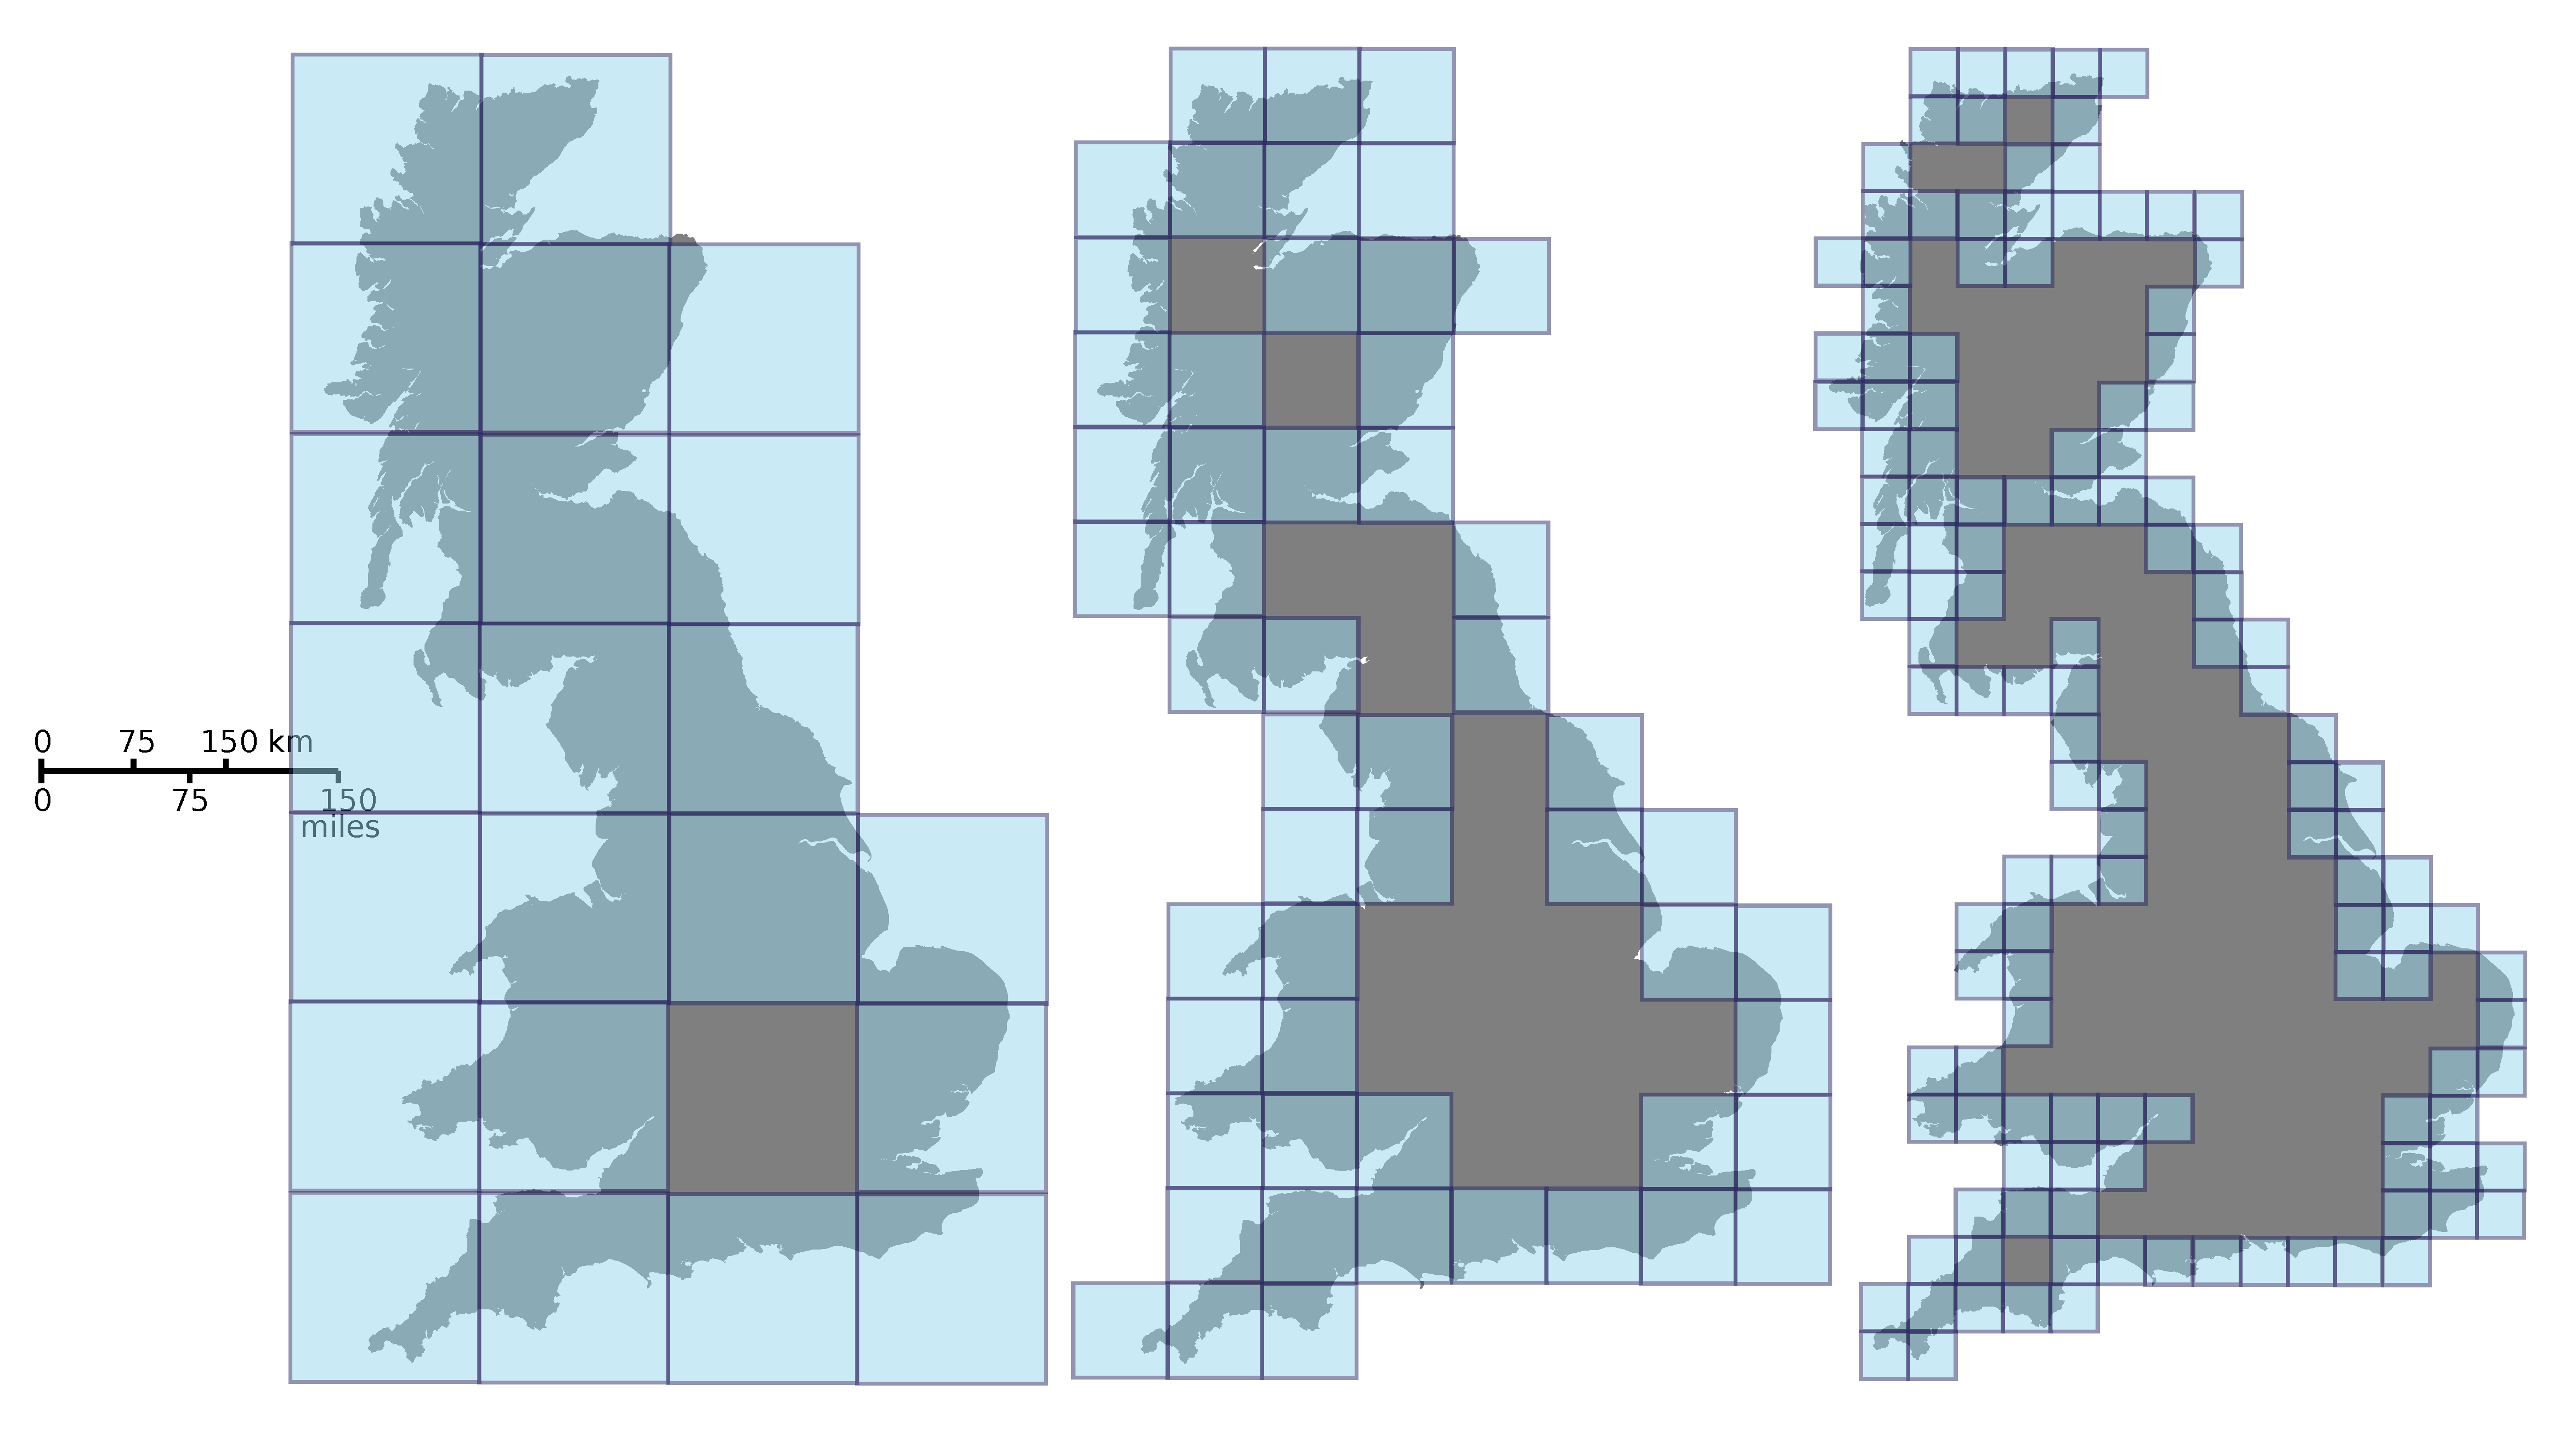
\includegraphics[width=\textwidth]{Great_Britain_Box.pdf}
    \caption{Aproximace box-counting dimenze pobřeží Velké Británie. Převzato z Wikipedia Commons, \url{https://en.wikipedia.org/wiki/Minkowski\%E2\%80\%93Bouligand\_dimension\#/media/File:Great\_Britain\_Box.svg}. Viz též \url{https://en.wikipedia.org/wiki/Minkowski\%E2\%80\%93Bouligand\_dimension}.}
    \label{fig:aproximace-delky-pobrezi-vb}
\end{figure}
Nyní se opět vrátíme k fraktálům a výpočtům jejich dimenze, čemuž jsme se věnovali již v sekci \ref{sec:fraktalni_dimenze} kapitoly \ref{chapter:uvod_do_fraktalu}, konkrétně \ref{subsec:dimenze-fraktalu}. Tentokrát však budeme postupovat přímo podle definice box-counting dimenze \ref{def:box-counting-dimenze}, tedy budeme zvlášť zkoumat horní a dolní box-counting dimenzi.
\begin{example}[Cantorovo diskontinuum]\label{ex:cantorovo-diskontinuum}
    Již jsme měli možnost se přesvědčit, že Cantorovo diskontinuum, označme $F$, má box-counting dimenzi $\ln{2}/\ln{3}$. Zkusme nyní výpočet zopakovat, avšak vzlášť vypočítáme $\lowerdimB{F}$ a $\upperdimB{F}$ podíváme se, zda se shodují.

    Jako první provedeme horní odhad. Je potřeba zvolit $\delta$ a na jeho základě dopočítat $N_\delta(F)$. V $k$-té iteraci, kde $k=0,1,2,\ldots$, vznikne obecně $2^k$ intervalů, každý o délce $(1/3)^k$, pokud zvolíme $3^{-k}<\delta\leqslant 3^{-k+1}$, pak intervaly o délce nejvýše $\delta$ tvoří $\delta$ pokrytí, přičemž $N_\delta(F)\leqslant 2^k$. Tedy celkově pro $\delta$-pokrytí všech intervalů bude potřeba nejvýše $N_\delta(F)\leqslant 2^k$ množin $I_1,I_2,\ldots,I_{N_\delta(F)}$ o průměru $3^{-k}<\diam{F_i}\leqslant 3^{-k+1}$ pro každé $i$. Z toho dostáváme
    \[\upperdimB{F}=\limsup_{\delta\to 0}\dfrac{\ln{N_\delta(F)}}{-\ln{\delta}}\leqslant\limsup_{\delta\to 0}\dfrac{\ln{2^k}}{-\ln{3^{-k+1}}}=\limsup_{\delta\to 0}\dfrac{k\ln{2}}{(k-1)\ln{3}}=\dfrac{\ln{2}}{\ln{3}}.\]
    Naopak pokud uvážíme intervaly délky $3^{-k-1}\leqslant\delta<3^{-k}$, pak každý z nich má neprázdný průnik s maximálně jedním intervalem $k$-té iterace $F$. Těch je, jak již víme, $2^k$, tedy intervalů $I_1,I_2,\ldots,I_{N_\delta(F)}$ bude nejméně $2^k$ pro pokrytí $F$, tzn. $N_\delta(F)\geqslant 2^k$. Tím dostáváme dolní odhad:
    \[\lowerdimB{F}=\liminf_{\delta\to 0}\dfrac{\ln{N_\delta()}}{-\ln{\delta}}\geqslant\liminf_{\delta\to 0}\dfrac{\ln{2^k}}{-\ln{3^{-k-1}}}=\liminf_{\delta\to 0}\dfrac{k\ln{2}}{(k+1)\ln{3}}=\dfrac{\ln{2}}{\ln{3}}.\]

    Protože $\lowerdimB{F}=\upperdimB{F}=\ln{2}/\ln{3}$, tak box-counting dimenze Cantorova diskontinua je $\dimB{F}=\ln{2}/\ln{3}$.
\end{example}